% =============================================================================
% Practical SAT Solving - Uebungsblatt 1
% Dozent: Prof. Dr. Carsten Sinz
% Autor: Erlind Sejdiu
% =============================================================================
\documentclass[11pt, a4paper]{article}

% --- Sprache und Layout ---
\usepackage[ngerman, provide=*]{babel}
\usepackage[utf8]{inputenc}
\usepackage[T1]{fontenc}
\usepackage{lmodern}
\usepackage{microtype}
\usepackage[left=2.0cm, right=2.0cm, top=1.8cm, bottom=1.8cm]{geometry}
\usepackage{parskip}

% --- Mathe und Tabellen ---
\usepackage{amsmath}
\usepackage{amssymb}
\usepackage{booktabs}
\usepackage{xcolor}

% --- Grafiken ---
\usepackage{tikz}
\usetikzlibrary{decorations.pathreplacing}

% --- Code Listings ---
\usepackage{listings}
\definecolor{codebg}{RGB}{248, 248, 248}
\definecolor{codeborder}{RGB}{225, 225, 225}
\definecolor{codegreen}{RGB}{0, 128, 0}
\definecolor{codeblue}{RGB}{0, 0, 180}

\lstset{
    language=C,
    backgroundcolor=\color{codebg},
    basicstyle=\ttfamily\fontsize{7.5pt}{8.8pt}\selectfont,
    breaklines=true,
    frame=single,
    rulecolor=\color{codeborder},
    keywordstyle=\color{codeblue}\bfseries,
    commentstyle=\color{codegreen}\itshape,
    numbers=left,
    numberstyle=\tiny\color{gray},
    numbersep=5pt,
    tabsize=4,
    showstringspaces=false,
    aboveskip=4pt,
    belowskip=4pt
}

% --- Hyperref ---
\usepackage{hyperref}
\hypersetup{
    colorlinks=true,
    linkcolor=black,
    citecolor=black,
    urlcolor=blue
}

\begin{document}

% --- Header ---
\begin{flushleft}
    \textbf{Practical SAT Solving} -- WS 2026/27 \hfill \textbf{Erlind Sejdiu \& Johannes Ott}\\
    Prof. Dr. Carsten Sinz \hfill Hochschule Karlsruhe (HKA)\\
    \rule{\textwidth}{0.4pt}
\end{flushleft}

\begin{center}
    {\Large\bfseries Übungsblatt 1: Aufgaben 3 \& 4}
\end{center}
\vspace{0.2em}

% =============================================================================
\section*{Aufgabe 3: Van-der-Waerden-Zahlen}
% =============================================================================

Die Zahlen $1, \dots, n$ sollen rot oder blau gefärbt werden, sodass keine $k$ Zahlen mit gleichem Abstand (z.\,B.\ $2, 4, 6$) alle dieselbe Farbe haben. Jede Zahl $i$ bekommt eine Variable $x_i$ (rot/blau), also $\#\text{Variablen} = n$.

So eine Folge $a, a+d, \dots, a+(k-1)d$ ist durch Startwert $a$ und Abstand $d$ festgelegt. Die Abbildung zeigt alle Folgen für $n = 9$, $k = 3$: Jede Zeile ist ein Abstand $d$, jedes blaue Kästchen ein möglicher Startwert.

\begin{center}
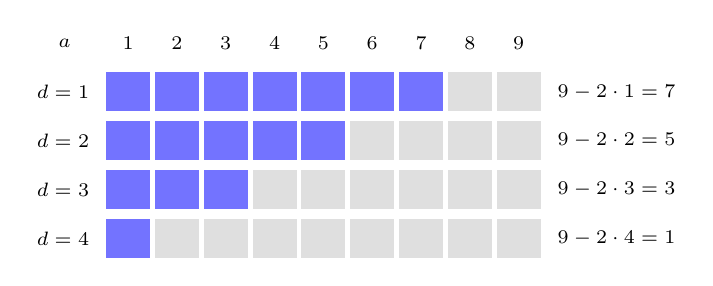
\begin{tikzpicture}[x=0.62cm, y=0.62cm, font=\scriptsize]
    \foreach \i in {1,...,9} \node at (\i, 0) {\i};
    \node at (-0.3, 0) {$a$};
    \foreach \d in {1,...,4} {
        \pgfmathtruncatemacro{\m}{9 - 2*\d}
        \foreach \i in {1,...,9} {
            \ifnum\i>\m
                \fill[gray!25] (\i-0.45, -\d-0.4) rectangle (\i+0.45, -\d+0.4);
            \else
                \fill[blue!55] (\i-0.45, -\d-0.4) rectangle (\i+0.45, -\d+0.4);
            \fi
        }
        \node[anchor=east] at (0.4, -\d) {$d=\d$};
        \node[anchor=west] at (9.6, -\d) {$9 - 2 \cdot \d = \m$};
    }
\end{tikzpicture}
\end{center}

Aus der Abbildung abgelesen: Pro Zeile gibt es $n - (k-1)d$ Startwerte, und es gibt $D = \left\lfloor \frac{n-1}{k-1} \right\rfloor$ Zeilen. Damit:
\begin{equation*}
    \#\text{Folgen} = \sum_{d=1}^{D} \bigl(n - (k-1)d\bigr) = nD - (k-1)\sum_{d=1}^{D} d = nD - (k-1)\frac{D(D+1)}{2}
\end{equation*}
Jede Folge liefert 2 Klauseln (nicht alle rot, nicht alle blau):
\begin{equation*}
    \boxed{\#\text{Klauseln} = 2 \cdot \#\text{Folgen} = 2nD - (k-1)D(D+1), \qquad D = \left\lfloor \frac{n-1}{k-1} \right\rfloor}
\end{equation*}
Probe ($n = 9$, $k = 3$, $D = 4$): $2 \cdot 9 \cdot 4 - 2 \cdot 4 \cdot 5 = 32$ (vgl.\ Folie 18).

\newpage
% =============================================================================
\section*{Aufgabe 4: Pythagoräische Tripel}
% =============================================================================

\subsection*{Teil 1: Lösung für die ersten 1000 Zahlen ($n = 1000$)}

Die Zahlen $1, \dots, 1000$ sollen rot oder blau gefärbt werden, sodass bei keinem Tripel mit $a^2 + b^2 = c^2$ alle drei Zahlen dieselbe Farbe haben. Für jedes Tripel werden zwei Klauseln erzeugt: $(x_a \lor x_b \lor x_c)$ und $(\neg x_a \lor \neg x_b \lor \neg x_c)$.

\begin{itemize}\setlength{\itemsep}{1pt}
    \item \textbf{Variablen:} $1000$
    \item \textbf{Tripel:} $881$
    \item \textbf{Klauseln:} $2 \times 881 = 1762$
    \item \textbf{Ergebnis:} Das Problem ist \textbf{SAT} (erfüllbar).
\end{itemize}

\paragraph{Solver-Skript (\texttt{Blatt1\_Aufgab4.c}):}
\begin{lstlisting}
/*
 * Kompilieren (Beispiel mit CaDiCaL, das IPASIR implementiert):
 *   gcc pythagoras_ipasir.c -I<cadical>/src <cadical>/build/libcadical.a -lstdc++ -lm
 */
#include <stdio.h>
#include <stdlib.h>
#include <math.h>
#include "ipasir.h"

static void klausel(void *s, int a, int b, int c) {
    ipasir_add(s, a);
    ipasir_add(s, b);
    ipasir_add(s, c);
    ipasir_add(s, 0);
}

int main(int argc, char **argv) {
    int n = argc > 1 ? atoi(argv[1]) : 30;

    void *solver = ipasir_init();               /* Solver anlegen */

    int anzahl = 0;
    for (int a = 1; a <= n; a++) {
        for (int b = a + 1; b <= n; b++) {
            long c2 = (long)a * a + (long)b * b;
            int c = (int)sqrtl((long double)c2);
            if (c > n) break;
            if ((long)c * c != c2) continue;
            klausel(solver,  a,  b,  c);        /* nicht alle blau */
            klausel(solver, -a, -b, -c);        /* nicht alle rot  */
            anzahl++;
        }
    }
    printf("n = %d: %d Tripel, %d Klauseln\n", n, anzahl, 2 * anzahl);

    /* 3. Loesen: 10 = SAT, 20 = UNSAT */
    int ergebnis = ipasir_solve(solver);

    if (ergebnis == 10) {
        printf("SAT Faerbung gefunden\n");
        if (n <= 50) {
            for (int i = 1; i <= n; i++)
                printf("%d: %s\n", i, ipasir_val(solver, i) > 0 ? "rot" : "blau");
        }
    } else if (ergebnis == 20) {
        printf("UNSAT keine Faerbung moeglich\n");
    }

    ipasir_release(solver);                     /* 5. Aufraeumen */
    return 0;
}
\end{lstlisting}

\paragraph{Programmausgabe für $n = 1000$:}
\begin{verbatim}
n = 1000: 881 Tripel, 1762 Klauseln
SAT Faerbung gefunden
\end{verbatim}

\paragraph{Alternative Lösung in Python:}
Dieses Skript schreibt die Klauseln in eine Datei \texttt{problem.cnf}, die man dann mit einem SAT-Solver lösen kann (z.\,B.\ \texttt{cadical problem.cnf}). Für $n = 1000$ kommen ebenfalls $881$ Tripel bzw.\ $1762$ Klauseln heraus.
\begin{lstlisting}[language=Python]
import math
import sys


def generate_cnf(n, filename):

    """
    Schaut mit jeder (sinnvollen) Kombination aus a und b, ob es ein c gibt,
    das unter n(1000) und ganzzahlig ist. Wenn ja, fuege es zu den Klauseln hinzu
    """

    clauses = []
    for a in range (1, n + 1):
        for b in range (a, n + 1):
            c2 =  a * a + b * b
            c = math.sqrt(c2)
            if (c.is_integer() and c <= n):
                c = int(c)
                clauses.append([a, b, c])

                clauses.append([-a, -b, -c])


    """
    Erstelle eine .cnf Datei mit den Klauseln
    """

    # DIMACS-Datei schreiben
    with open(filename, "w") as f:
        f.write(f"p cnf {n} {len(clauses)}\n")
        for clause in clauses:
            f.write(" ".join(map(str, clause)) + " 0\n")

    print(f"CNF erstellt: {filename}")
    print(f"Variablen:    {n}")
    print(f"Klauseln:     {len(clauses)}")
    print(f"Tripel:       {len(clauses) // 2}")


if __name__ == "__main__":
    n = int(sys.argv[1]) if len(sys.argv) > 1 else 100

    generate_cnf(n, "problem.cnf")
\end{lstlisting}

\newpage
\subsection*{Teil 2: Abschätzung von Variablen und Klauseln bis zur Zahl \texorpdfstring{$n$}{n}}

Jede Zahl $1 \le i \le n$ erhält eine Variable, also $\#\text{Variablen}(n) = n$.

Jedes Tripel ist durch das Paar $(a, b)$ mit $a < b \le n$ eindeutig bestimmt und liefert 2 Klauseln. Es gibt höchstens $\binom{n}{2}$ solcher Paare, also:
\begin{equation*}
    \boxed{\#\text{Klauseln}(n) \le 2\binom{n}{2} = n(n-1) = \mathcal{O}(n^2)}
\end{equation*}


\end{document}
